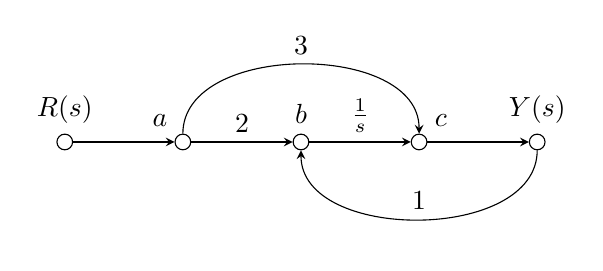
\begin{tikzpicture}[
    terminal/.style 2 args={draw,circle,inner sep=2pt,label={#1:#2}},
    amark/.style={
    ->,
    >=stealth,
    every node/.append style={above,midway}
    },
    node distance=2cm
]

%Draw the connections
\node[terminal={above}{$R(s)$}] (a) at (0,0) {};
\node[terminal={above left}{$a$}] (b) at (1.5,0) {};
\node[terminal={above}{$b$}] (c) at (3,0) {};
\node[terminal={above right}{$c$}] (d) at (4.5,0) {};
\node[terminal={above}{$Y(s)$}] (e) at (6,0) {};
%Draw the connections
\draw[amark](a) to (b);
\draw[amark] (b) to node{$2$}(c);
\draw[amark] (c) to node{$\frac{1}{s}$} (d);
\draw[amark] (b) to [bend left=90] node{$3$}(d);
\draw[amark] (d) to (e);
\draw[amark] (e) to[bend left=90] node{$1$}(c);


\end{tikzpicture}

